%! Author = t
%! Date = 3/12/24

% Preamble
\documentclass[11pt]{article}
\usepackage{graphicx}
\usepackage{amsmath}

\title{Assignment Chapter-2}
\author{Timofey Brayko\\1820243088}
\begin{document}
    \maketitle

    \section{Task}
    A noiseless 4-kHz channel is sampled every 1 msec.
    What is the maximum data rate?
    How does the maximum data rate change if the channel is noisy,
    with a signal-to-noise ratio of 30 dB?
    \subsection{Solution}
        \begin{enum}
            \item \paragraph{1.} Let us assume that binary data are transmitted via the connection.
                Due to Nyquist rule bit rate should be 2 times larger than available channel bandwidth.
                Thus:
                \begin{equation}
                    C = 2H \times log_{2}(v) = 2 \times 4 \times 10^3 \times log_{2}2 = 8 Kbps
                \end{equation}
            \item \paragraph{2.} Due to the Shannon formula we got the following formula:
                \begin{equation}
                    C = H \times log_2(1+S/N) = 4 \times 10^3 \times log_2(1 + 10^{30/10}) \approx 39.87 Kbps
                \end{equation}
        \end{enum}
        \paragraph{Answers:} 1)8 Kbps; 2)39.87 Kbps

    \newpage

    \section{Task}
    \begin{figure}[htp]
		\centering
		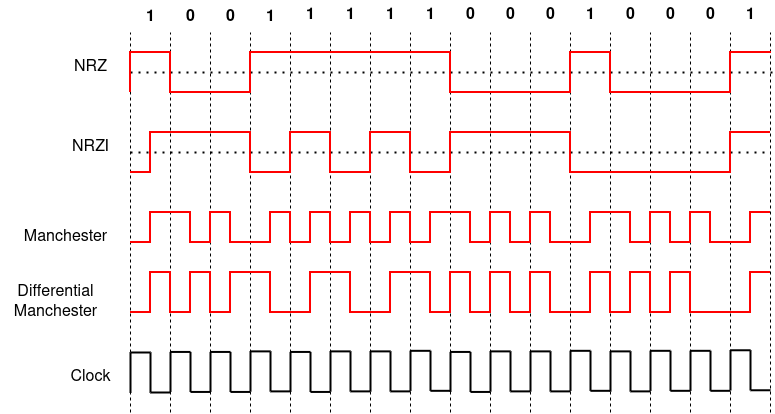
\includegraphics[width=12cm]{figs/Signals}
		\caption{Solution}
	\end{figure}

    \section{Task}
        What are the disadvantages of Manchester Encoding?

    \subsection{Answer}
        \begin{enumerate}
            \item It requires much more bandwidth
            \item Manchester encoding has a lower bit in comparison with others.So it takes more time to transmit data.
            \item Because of frequent voltage transitions, on the long distances the signal loses its strength
            \item At least we have one transition per bit time and maximum two transitions
        \end{enumerate}


        At least one transition per bit time and possibly two \\
        Bandwidth inefficient: 50\% \\

    \section{D}
        A total of four stations perform code division multiple access CDMA communication.
        The chip sequences of the four stations are: \\
            A: (-1 -1 -1 +1 +1 -1 +1 +1) \\
            B: (-1 -1 +1 -1 +1 +1 +1 -1) \\
            C: (-1 +1 -1 +1 +1 +1 -1 -1) \\
            D: (-1 +1 -1 -1 -1 -1 +1 -1) \\
        Station X now receives such a chip sequence: (-1 +1 -3 +1 -1 -3 +1 +1).
        Which stations transmitted, and which bits did each one send?
        \subsection{Solution}
    In order to define which station take part in communication,
    we will compute the dot product of the result and
    each station chip sequence, and divide by its length.

        \[
            \begin{pmatrix}
                -1 & -1 & -1 & 1 & 1 & -1 & 1 & 1 \\
                -1 & -1 & 1 & -1 & 1 & 1 & 1 & -1 \\
                -1 & 1 & -1 & 1 & 1 & 1 & -1 & -1 \\
                -1 & 1 & -1 & -1 & -1 & -1 & 1 & -1
              \end{pmatrix} \;
              \times
              \begin{pmatrix}
                -1\\ +1\\ -3\\ +1\\ -1\\ -3\\ +1\\ +1
              \end{pmatrix}
                =
              \begin{pmatrix}
                  1 \\ -1 \\ 0 \\ 1
              \end{pmatrix}
        \]

    Thus, only $\bf A, B,$ and $\bf D$ stations took part in data transition
    \paragraph{Answer:} A + $\overline{B}$ + D

\end{document}
